%==============================================================================
\chapter{Model validation: encoding $\Ca$ transient variations to map pharmaceutical modulations from the whole-cell to whole-organ in the healthy rat 
heart}\label{cha:chapter6}
%==============================================================================
%
%
%
\begin{remark}{Outline}
    In this chapter, we use the personalised healthy control SHAM rat model to map drug effects across scales. \todo{write}
\end{remark}


%
%
%
\section{Encoding calcium transient variations}
We used a $4$-feature parametric representation of the calcium transient that maps to common experimentally measured features. The calcium transient was characterised using diastolic concentration (\acs{DCA}), amplitude (\acs{AMPL}), time to peak concentration (\acs{TP}) and time to half-relaxation from peak concentration (\acs{RT$_{50}$}) features. We wish to sample random sets of these features such that the final samples will uniformly cover the feature space, in order to possibly cover both healthy and pathological calcium transient phenotypes. For this purpose, we used linear weighs to scale each of the four features from a representative calcium transient. This parametric encoding of calcium transient variation ensured that all transients maintained a characteristic calcium transient morphology.

\vspace{0.2cm}
The specific implementation of this scaling strategy is presented in Alg.~\ref{alg:cascaling}. Note that \texttt{features} function returns the set of four features given an input calcium transient; \texttt{concatenate} function returns a $1$D array obtained as the horizontal stack of the given input row $1$D arrays; \texttt{linear\_interpolator} function returns a function whose call method uses $1$D linear interpolation to find the value of new points.

\begin{algorithm}
    \caption{Scaling a representative calcium transient (y:=$\Cai(t)$) using linear interpolation.}\label{alg:cascaling}
    \begin{algorithmic} 
    \REQUIRE $t=(t_1,\,\dots,\,t_N),\,y=(y_1,\,\dots,\,y_N),\,\,\textrm{with}\quad t_i,\,y_i\ge 0\,\,\forall\,\,i=1,\dots,\,N$ \\ $p=(p_1,\,\dots,\,p_4),\,\,\textrm{with}\quad p_i\ge 0\,\,\forall\,\,i=1,\dots,\,4$
    \ENSURE $y_{new}\,\,|\,\,(\textrm{features}(t,\,y_{new}))_{i} = p_i\cdot(\textrm{features}(t,\,y))_{i}\quad\forall\,\,i=1,\dots,4$ \\ $\textrm{where}\,\,\textrm{features}(t,\,y) = (\dca,\,\ampl,\,\tp,\,\rtf)$ \\ \vspace{0.2cm}
    \STATE $\dca\,\,\leftarrow\,\,(\textrm{features}(t,\,y))_1$
    \STATE $y_{new}\,\,\leftarrow\,\,p_1\cdot\dca + p_2\cdot(y-\dca)$
    \STATE $i_{max}\,\,\leftarrow\,\,\argmax\limits_{i=1,\dots,\,N}{y}$
    \STATE $T \leftarrow t_{N}$ \\
    \vspace{0.2cm}
    \IF{$\,\, p_3\cdot(t_{i_{max}} - t_{1}) + p_4\cdot(t_{N}-t_{i_{max}})\le T\,\,$}
    \STATE $s\,\,\leftarrow\,\,(p_3 - p_4)\cdot t_{i_{max}}$
    \STATE $t_{tmp}\,\,\leftarrow\,\,\textrm{concatenate}(p_3\cdot (t_{1},\,\dots,\,t_{i_{max}}),\,\,(p_4\cdot t_{i_{max}+1}+s,\,\dots,\,p_4\cdot t_{N-1}+s),\,\,(t_{N}))$
    \STATE $f\,\,\leftarrow\,\,\textrm{linear\_interpolator}(t_{tmp},\, y_{new})$
    \STATE $y_{new}\,\,\leftarrow\,\,f(t)$
    \ELSE
    \PRINT ``Not a valid scaling! Returning original calcium curve."
    \STATE $y_{new}\,\,\leftarrow\,\,y$
    \ENDIF
    \RETURN $y_{new}$
    \end{algorithmic}
\end{algorithm}

\vspace{0.2cm}
Fig.~\ref{fig:algintopractice} shows how the algorithm works and how new random calcium transients can be generated.

\begin{figure}[!ht]
    \myfloatalign
    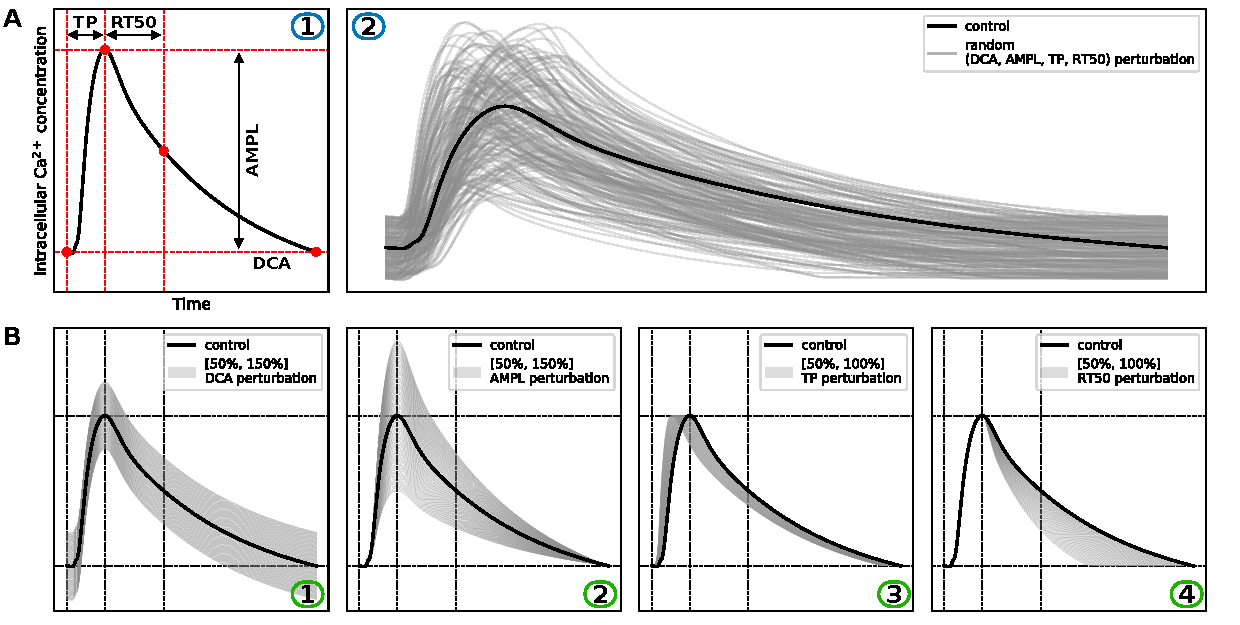
\includegraphics[width=\textwidth]{figures/chapter06/ca_biomarkers_and_scaling_explained_with_labels.pdf}
    \caption{A $4$-feature parametric representation of the calcium transient. (A.1) The calcium transient is described by four relevant quantities: diastolic concentration ($\dca$), amplitude ($\ampl$), time to peak concentration ($\tp$) and time to half-relaxation from peak concentration ($\rtf$). (B.1--4) Each of the $4$ calcium features can be scaled independently to produce a new calcium transient. (A.2) All the features can be scaled at the same time to produce many different new calcium transients.}
    \label{fig:algintopractice}
\end{figure}

\vspace{0.2cm}
An important property of this calcium scaling strategy is that the features scale linearly with the scaling coefficient used, as shown in Fig.~\ref{fig:scalersvscafeatures}. This allows us to randomly sample the scalar parameters that encode the calcium transient from a space filling design (e.g. a Latin hypercube) while generating samples that cover the full feature space. Having a training dataset with input parameters that uniformly cover the high-dimensional parameter space also helps Gaussian process emulators training while at the same time improving their prediction accuracy.

\begin{figure}[!ht]
    \myfloatalign
    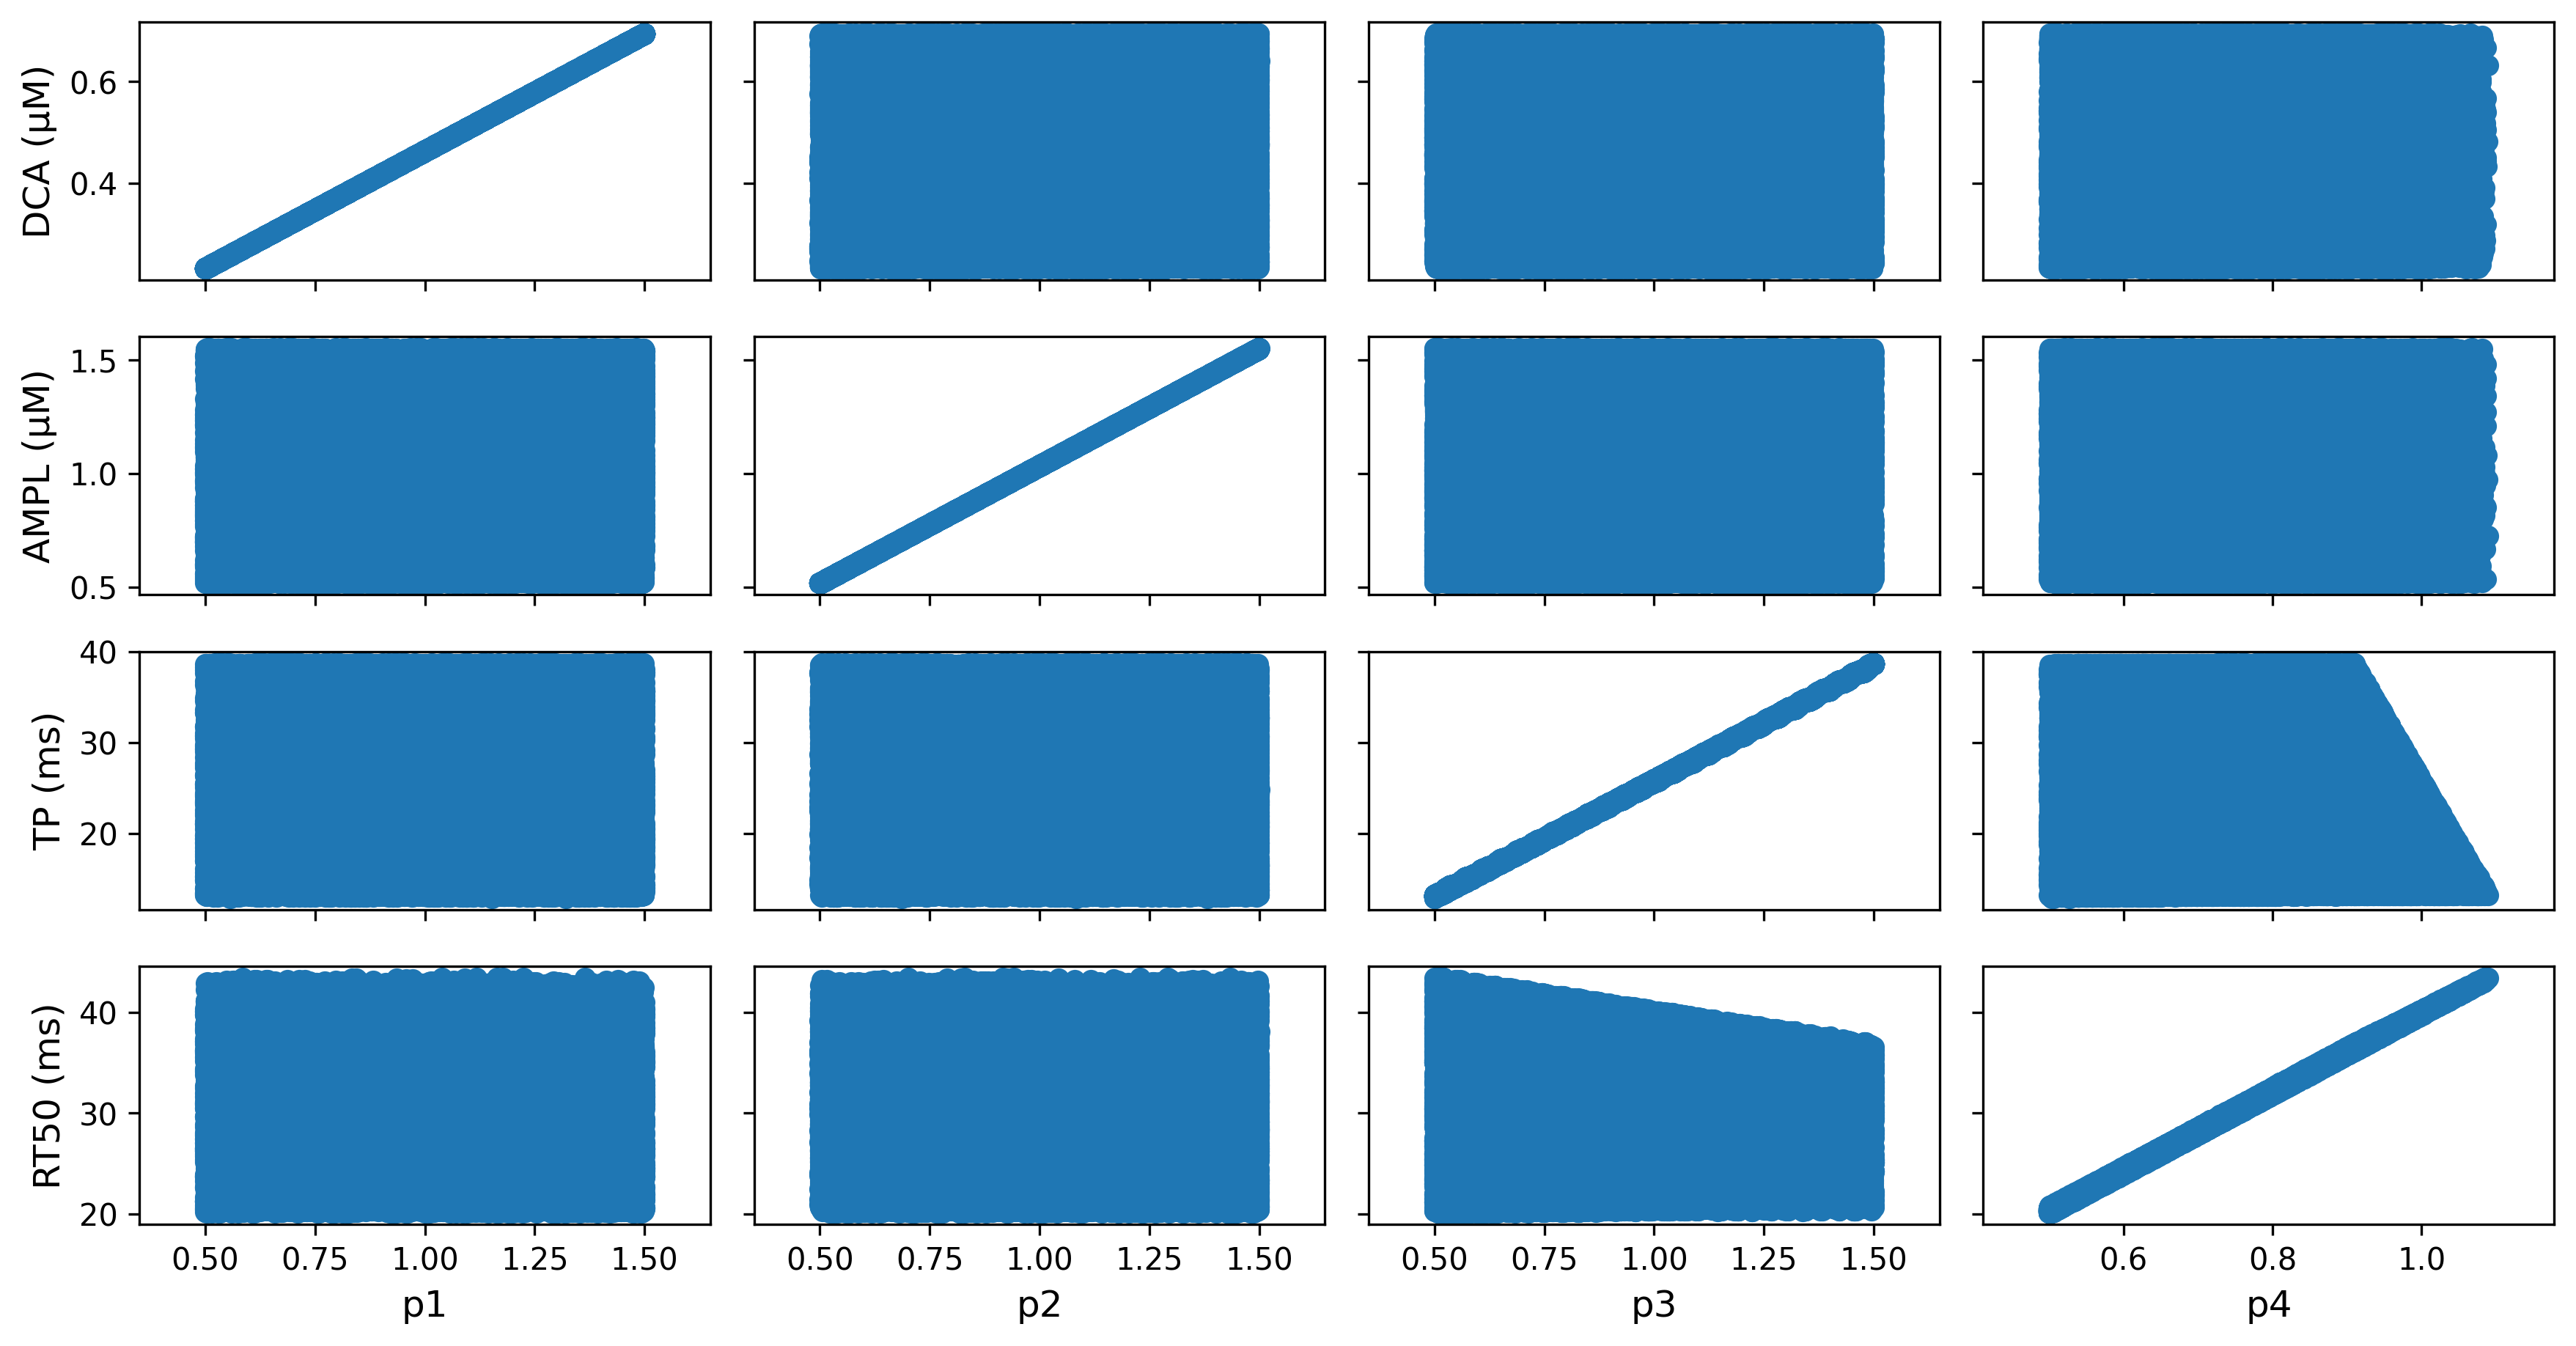
\includegraphics[width=\textwidth]{figures/chapter06/p_vs_b.png}
    \caption{Calcium transient features linearly scale with their respective scaling coefficients. Example showing $[\SI{50}{\percent},\,\SI{150}{\percent}]$ perturbation for all the calcium features but $\rtf$, which undergoes a $[\SI{50}{\percent},\,\SI{110}{\percent}]$ perturbation.}
    \label{fig:scalersvscafeatures}
\end{figure}

\vspace{0.2cm}
The employed ionic model generates a calcium transient for a fixed pacing rate ($\SI{6}{Hz}$), so that it occurs within a fixed time span. At physiological pacing rates, the rat calcium transient never reaches an equilibrium in diastole, so that during a calcium transient time is spent rising or relaxing. As the cell is paced at a fixed cycle length, the sum of time to peak and relaxation time is capped. This means that one cannot increase without the other decreasing, and independent perturbation of $\tp$ and $\rtf$ can only decrease. If relaxation does interdependently slow, this will mean that the cell will not have enough time to fully relax, and this effect is captured by elevating $\dca$ while decreasing $\ampl$. From an algorithmic view point, not all the randomly picked calcium features' scaling coefficient sets will therefore be viable. The ``if" statement in Alg.~\ref{alg:cascaling} controls this behaviour by discarding all those curves that decay outside the fixed time interval without fully repolarising.

\vspace{0.2cm}
The existing coupling between $\tp$ and $\rtf$ calcium features manifests as regions of the feature space that can not be captured by our calcium transient scaling strategy. These are indiecated by the blank triangels in the $p_3$-vs-$\rtf$ and $p_4$-vs-$\tp$ subplots, visible in Fig.~\ref{fig:scalersvscafeatures}.



%
%
%
\section{Model validation}\label{sec:validmethod}
To test if the rat heart contraction model and its probabilistic surrogate can predict how changes in calcium transients impact the whole heart function, we validated the computational framework by comparing qualitative measurements and predictions of changes in cardiac mechanics in the presence of drugs that manipulate the calcium transient. This provides a multi-scale test on the ability of the model to map from changes in ion channels conductances to changes in calcium transient and the resulting changes in whole heart function.

\vspace{0.2cm}
Briefly, we selected $8$ compounds, which were well characterised for multiple ion channels and for which we could find whole organ measurements from literature, from the \textit{comprehensive in vitro proarrhythmia assay} (\acs{CiPA})~\cite{Park:2019} official list, namely bepridil, chlorpromazine, diltiazem, mexiletine, nifedipine, ranolazine, sotalol and verapamil, and we described their action at the cell level using a 4-channel description, namely I\textsubscript{Na}, I\textsubscript{to}, I\textsubscript{K1} and I\textsubscript{CaL}. I\textsubscript{Kr} channel was not included as it has a small amplitude in rats myocytes~\cite{Wymore:1997} and so was not included in the employed rat cell model~\cite{Gattoni:2017}.

\vspace{0.2cm}
The affinity of each compound for each channel was taken from CiPA project datasets~\cite{Li:2018, Li:2019}, summarised in Table~\ref{tab:drugporeblock}.
%
\begin{table}[!ht]
    \myfloatalign
    \begin{tabularx}{\textwidth}{lllll}
    \toprule
    \tableheadline{Drug} & \multicolumn{4}{c}{\spacedlowsmallcaps{Ion channel}} \\
    \midrule
    & \tableheadline{I\textsubscript{Na}} & \tableheadline{I\textsubscript{to}} & \tableheadline{I\textsubscript{K1}} & \tableheadline{I\textsubscript{CaL}} \\
    \midrule
    \tableheadline{bepridil}  & & & & \\
    $IC_{50}$ ($\SI{}{\nano\Molar}$)     & $2.93\cdot10^{3}$ & $8.59\cdot10^{3}$ & - & $2.81\cdot10^{3}$ \\
    h                               & $1.16$ & $3.54$ & - & $0.65$ \\ \midrule
    \tableheadline{chlorpromazine}  & & & & \\
    $IC_{50}$ ($\SI{}{\nano\Molar}$)     & $4.54\cdot10^{3}$ & $1.76\cdot10^{7}$ & $9.27\cdot10^{3}$ & $8.19\cdot10^{3}$ \\
    h                               & $2.00$ & $0.37$ & $0.69$ & $0.84$ \\ \midrule
    \tableheadline{diltiazem}       & & & & \\
    $IC_{50}$ ($\SI{}{\nano\Molar}$)     & $1.11\cdot10^{5}$ & $2.82\cdot10^{9}$ & - & $1.12\cdot10^{2}$ \\
    h                               & $0.70$ & $0.17$ & - & $0.71$ \\ \midrule
    \tableheadline{mexiletine}      & & & & \\
    $IC_{50}$ ($\SI{}{\nano\Molar}$)     & - & - & - & $3.82\cdot10^{4}$ \\
    h                               & - & - & - & $1.03$ \\ \midrule
    \tableheadline{nifedipine}      & & & & \\
    $IC_{50}$ ($\SI{}{\nano\Molar}$)     & $2.84\cdot10^{4}$ & - & - & $1.15\cdot10^{1}$ \\
    h                               & $1.11$ & - & - & $0.67$ \\ \midrule
    \tableheadline{ranolazine}      & & & & \\
    $IC_{50}$ ($\SI{}{\nano\Molar}$)     & $6.88\cdot10^{4}$ & - & - & - \\
    h                               & $1.42$ & - & - & - \\ \midrule
    \tableheadline{sotalol}         & & & & \\
    $IC_{50}$ ($\SI{}{\nano\Molar}$)     & $1.14\cdot10^{9}$ & $\SI{4.31e7}{}$ & $3.05\cdot10^{6}$ & $7.06\cdot10^{6}$ \\
    h                               & $0.51$ & $0.66$ & $1.20$ & $0.87$ \\ \midrule
    \tableheadline{verapamil}       & & & & \\
    $IC_{50}$ ($\SI{}{\nano\Molar}$)     & - & $1.34\cdot10^{4}$ & $3.49\cdot10^{8}$ & $2.02\cdot10^{2}$ \\
    h                               & - & $0.82$ & $0.27$ & $1.10$ \\
    \bottomrule                          
    \end{tabularx}
    \caption{$\icf$ and Hill coefficient values describing the affinity of eight CiPA compounds with the I\textsubscript{Na}, I\textsubscript{to}, I\textsubscript{K1} and I\textsubscript{CaL} ion channels. The dash symbol indicates that the specific compound has no inhibitory effect on the respective ion channel. Values taken from~\cite{Li:2018, Li:2019}.}
    \label{tab:drugporeblock}
\end{table}

\noindent
The affinity is described by the Hill coefficient $h$ and the half-maximal inhibitory concentration $\icf$ values of a Hill-type relationship which gives the fraction of blocked current $B$ as a function of the drug concentration $C$, also known as pore block model:
%
\begin{equation}
    B = \frac{1}{1+\left(\frac{C}{\icf}\right)^h}
\end{equation}

\noindent
For each given drug, we calculated $B$ for each channel when $C$ was set to equally-spaced values in a log-molar space. By subtracting the obtained $B$ values from $1$, we obtained a matrix of scaling coefficients for the channels' conductances, representing the fractions of active channels in the presence of the drugs at different concentrations. We tested $13$ equally-spaced drug concentrations ($-\log{\SI{}{\Molar}}$) in the range $[4,\,10]$ (extremes included), which corresponded to drugs concentrations between $\SI{e-10}{\Molar}$ and $\SI{e-4}{\Molar}$. We then run the Gattoni et al.~\cite{Gattoni:2017} model by scaling the ion channels conductances to simulate the action of different concentrations of each drug at the cell level and collected the resulting calcium transients (last beat curves of stead-state, $5000$ beats simulations). An example of calcium transients obtained after simulating the effect of verapamil is provided in Figure~\ref{fig:calciumverapamil}

\begin{figure}[!ht]
    \myfloatalign
    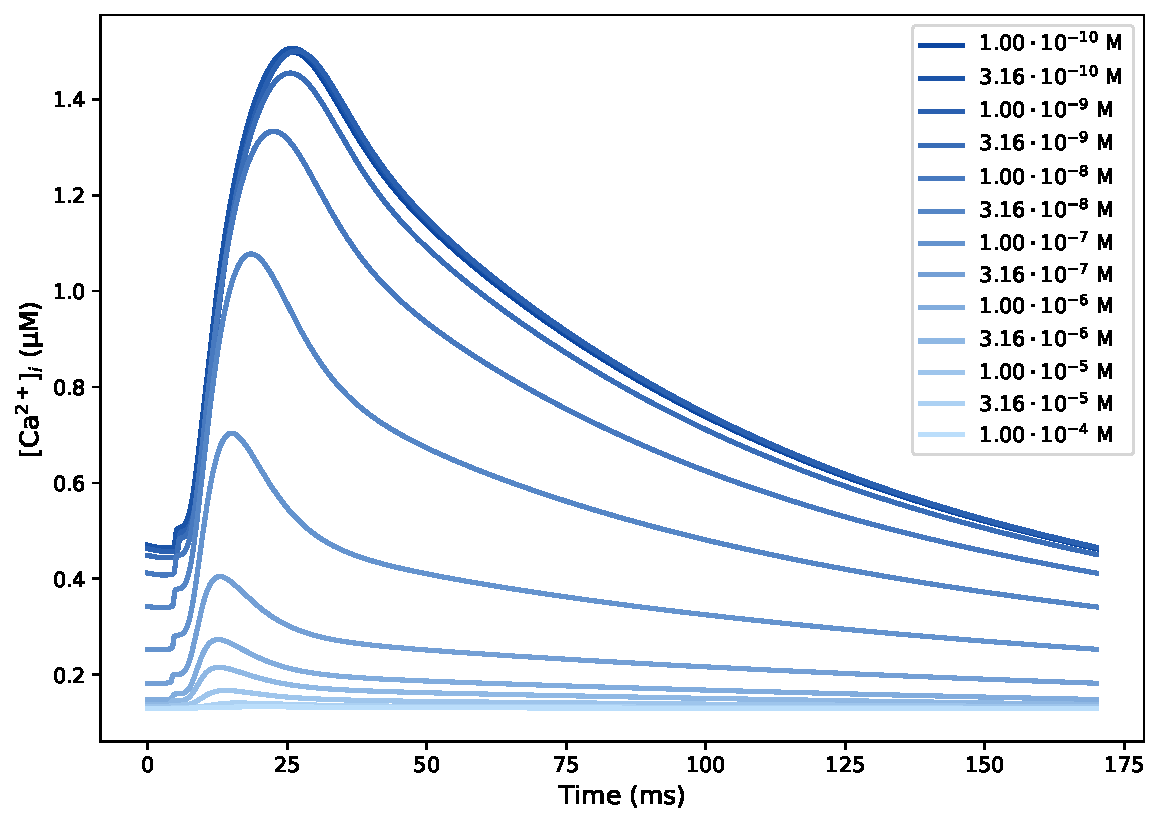
\includegraphics[width=0.8\textwidth]{figures/chapter06/verapamil_calcium_curve_drug.pdf}
    \caption{The effect of verapamil on intracellular calcium transient. Gattoni et al.~\cite{Gattoni:2017} model is run using different ion channels conductances' scaling coefficients to simulate the effect of different concentrations (blue colour variants) of the example drug considered.}
    \label{fig:calciumverapamil}
\end{figure}


\noindent
The used approach simulates the drug induced changes in calcium transients, thereby overcoming the issue when no directly recorded calcium transients are available. In so doing, we created a fully simulated map from drug properties to whole organ function. As the calcium transients obtained in the presence of the drug at different concentrations can be encoded by the presented $4$ features of interest ($\dca$, $\ampl$, $\tp$ and $\rtf$), the same $4$ features' dose-response curves can be plotted as well. These are shown in~Figure~\ref{fig:cafeatsverapamilrespcurve}.

\begin{figure}[!ht]
    \myfloatalign
    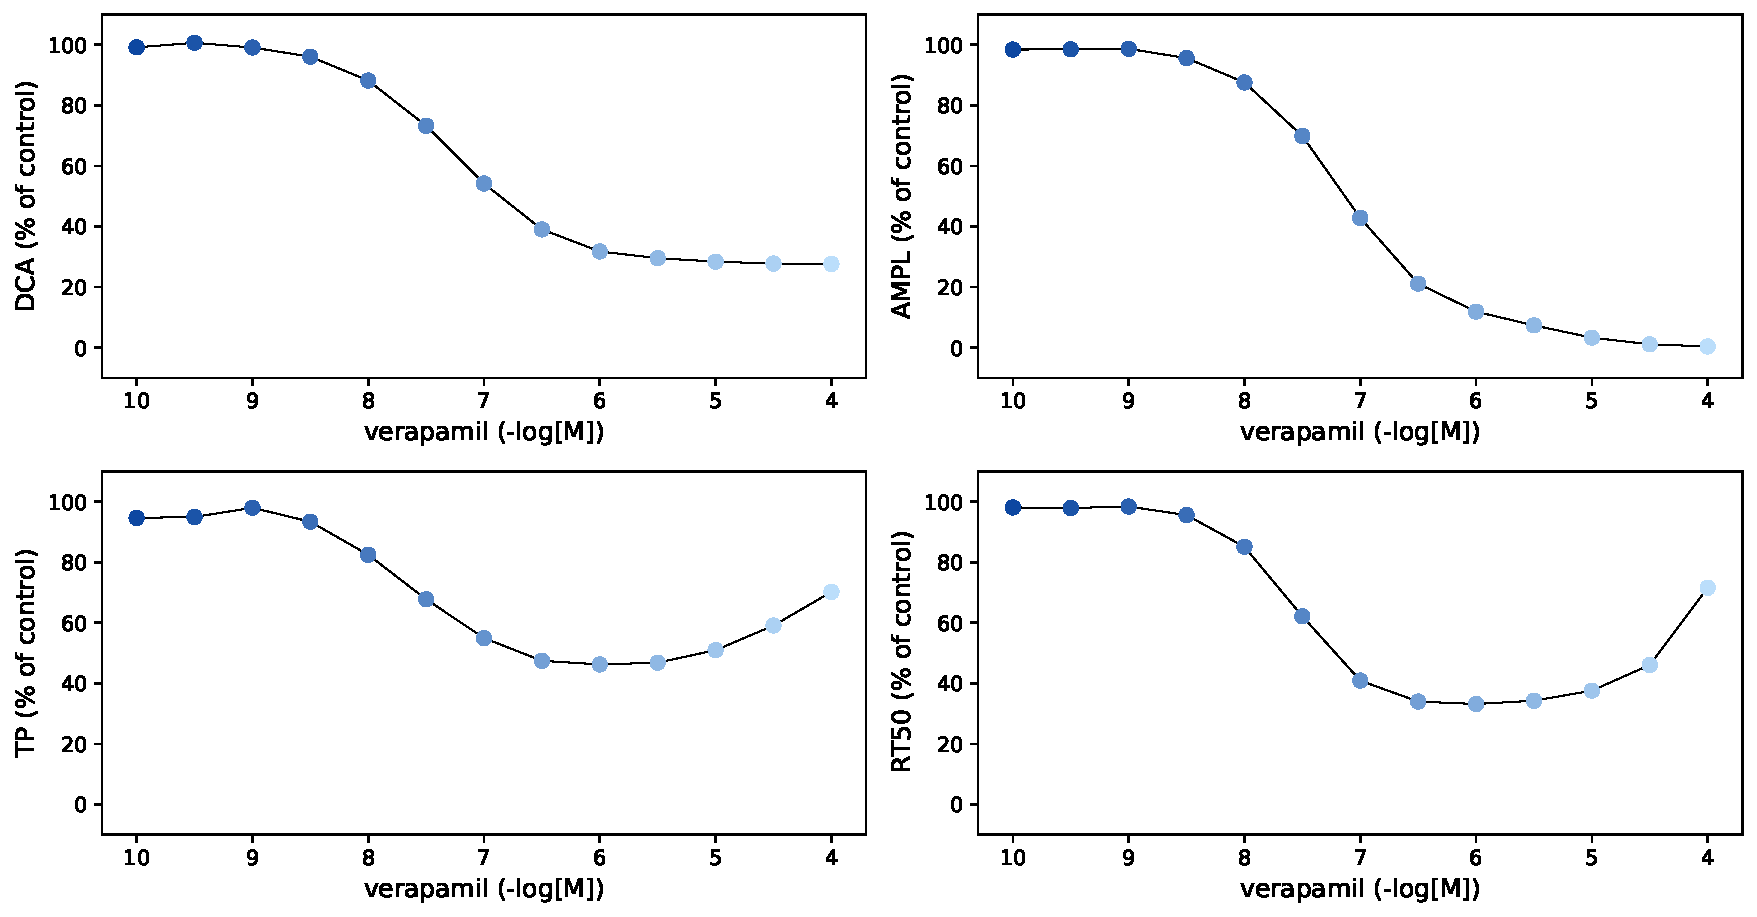
\includegraphics[width=\textwidth]{figures/chapter06/verapamil_dose_calcium_response_curve_drug.pdf}
    \caption{Calcium transient features dose-response curves. Calcium transient features are extracted from perturbed calcium transients and plotted against the respectively simulated drug concentrations.}
    \label{fig:cafeatsverapamilrespcurve}
\end{figure}

\noindent
We can notice that in the $\tp$ and $\rtf$ cases the response is not following a fully logistic trend on the right branches. This is because for high drug concentrations we have seen (Figure~\ref{fig:calciumverapamil}) that the calcium signal had almost vanished, making the analysis of these curves challenging.


\vspace{0.2cm}
We finally used the full multi-scale healthy rat model (Section) to simulate the LV features values using as an input the obtained calcium transients and the remaining parameters fixed to the SHAM rat model reference values. This allowed us to obtain the LV features' change from baseline values in a dose-dependent manner. PeakP, maxdP and mindP features' simulated responses to different doses of all the tested drugs are reported in Figure~\ref{fig:LVfeatsalldrugsrespcurves}

\begin{figure}[!ht]
    \myfloatalign
    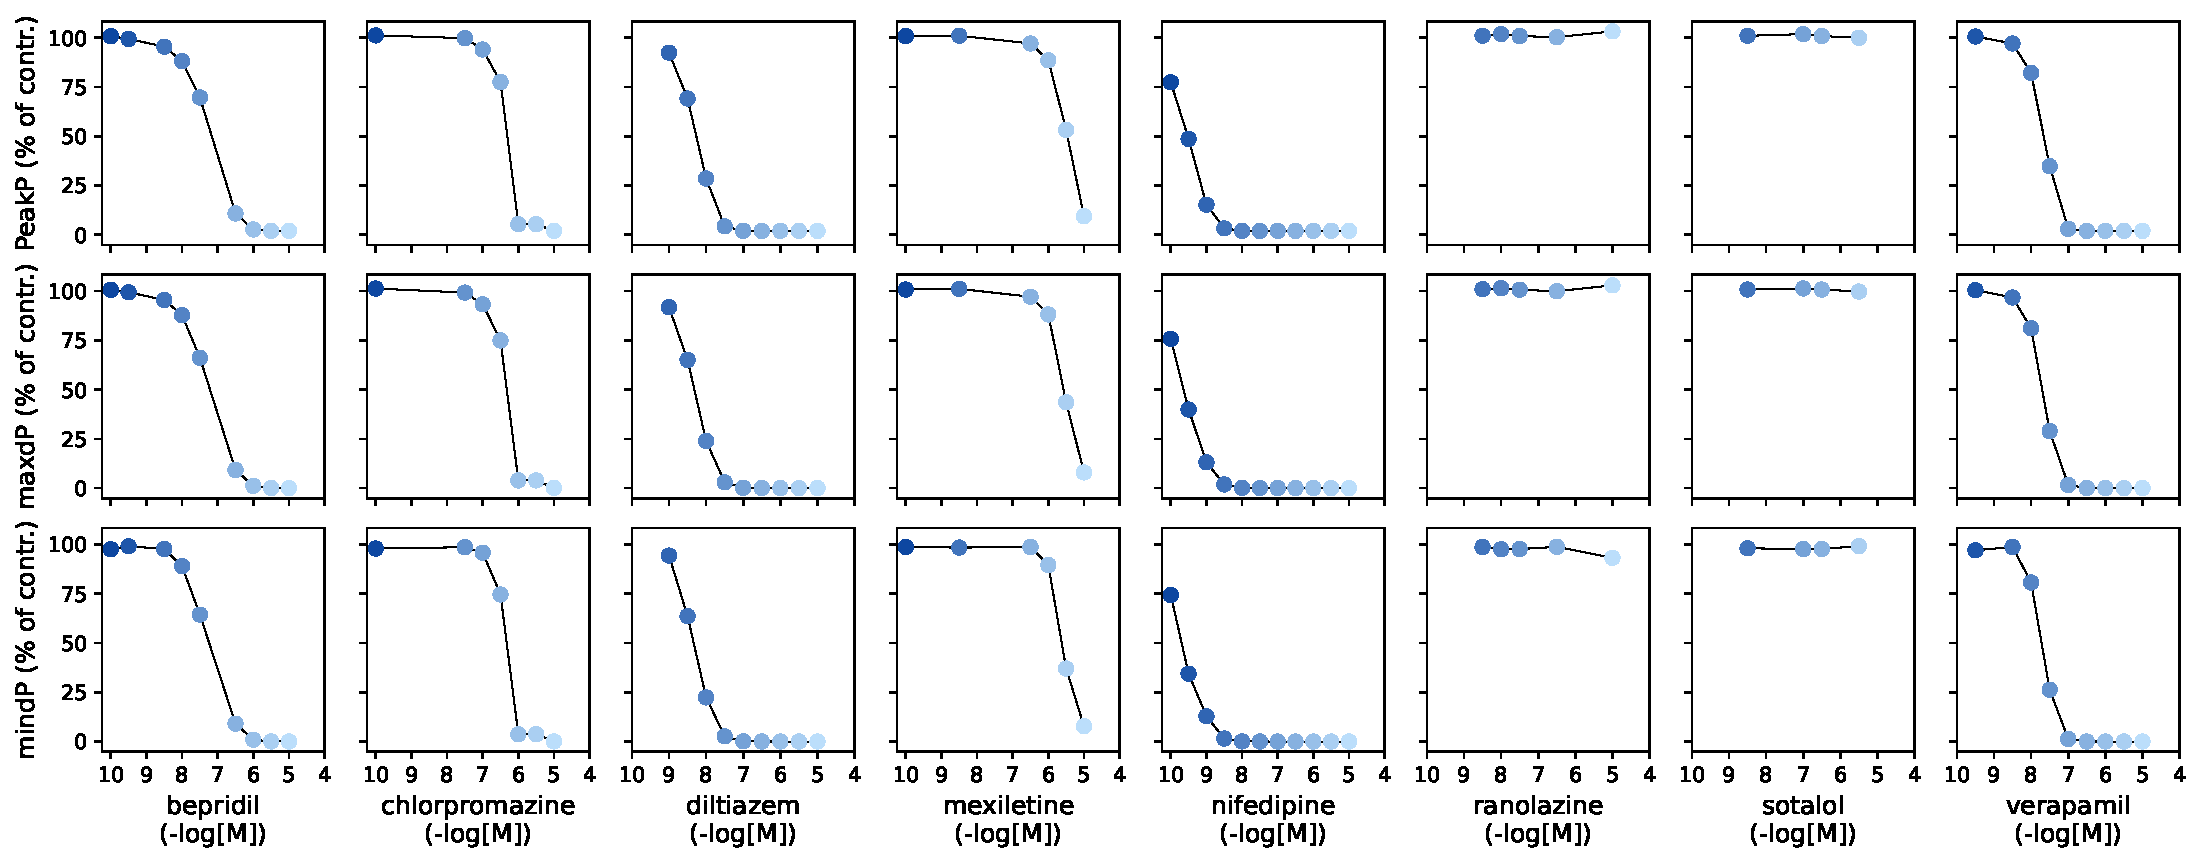
\includegraphics[width=1\textwidth]{figures/chapter06/lvp_features_responses_to_all_drugs.pdf}
    \caption{LV pressure features' dose-response curves for the eight CiPA compounds. Simulated PeakP, maxdP and mindP features are given as percentages of the respective control values, and are displayed as dots in blue variants colour-coded with the drug doses. \todo{improve}}
    \label{fig:LVfeatsalldrugsrespcurves}
\end{figure}

\noindent
These features' qualitative responses after \textit{in silico} drug ``administration'' were compared to qualitative changes in the same LV features observed after drugs administration in literature experimental studies performed on either conscious, or Langendorff-perfused or working healthy rat heart preparations. These experimental changes were either recorded after a single dose in the pre-ischemic phase of an ischemia-reperfusion experiment, or in a dose-dependent manner, and are summarised in Table~\ref{tab:drugvalidationrefs}.

\begin{table}[!ht]
    \myfloatalign
    \begin{tabular}{lcccl}
    \hline
    \textbf{Drug}           & \multicolumn{3}{c}{\textbf{LV feature}} & \textbf{References} \\
    \hline
    & PeakP & maxdP & mindP & \\
    \hline
    bepridil       & $\downarrow$ & $-$ & $-$ & \cite{Leiris:1984, Amsterdam:1988, Huizer:1987} \\
    chlorpromazine & $\downarrow$ & $-$ & $-$ & \cite{Katsuoka:1989, Langslet:1971, Sakai:2017} \\
    diltiazem      & $\downarrow$ & $\downarrow$ & $\downarrow$ & \cite{Flaim:1982, Koltai:1989, Dong:1997} \\
    mexiletine     & $\leftrightarrow$ & $\downarrow$ & $-$ & \cite{Kamiyama:1995, Hesketh:2020, Marshall:1981} \\
    nifedipine     & $\downarrow$ & $\downarrow$ & $\downarrow$ & \cite{Dong:1997, Saponara:2007, Nishimura:1992} \\
    ranolazine     & $\leftrightarrow$ & $\leftrightarrow$ & $\leftrightarrow$ & \cite{Wang:2007, Hwang:2009, Wang:2019} \\
    sotalol        & $\downarrow$ & $\downarrow$ & $\leftrightarrow$ & \cite{Mackin:2019, Peralta:2000, Hoffmeister:1988} \\
    verapamil      & $\downarrow$ & $\downarrow$ & $\downarrow$ & \cite{Simonovic:2019, Stojic:2017, Kolar:1990} \\
    \hline
    \end{tabular}
    \caption{Qualitative change in three LV pressure features observed in literature rat experiments for eight different CiPA compounds. Down-facing arrow means that the specific LV feature decreases from its control value with the specific drug; left-right arrow means that the drug has no effect on that feature; dash symbol means that the specific information could not be retrieved from literature.}
    \label{tab:drugvalidationrefs}
\end{table}


\noindent
The entire validation workflow is summarised in Fig.~\ref{fig:validationschematic}.

\begin{figure}[!ht]
    \myfloatalign
    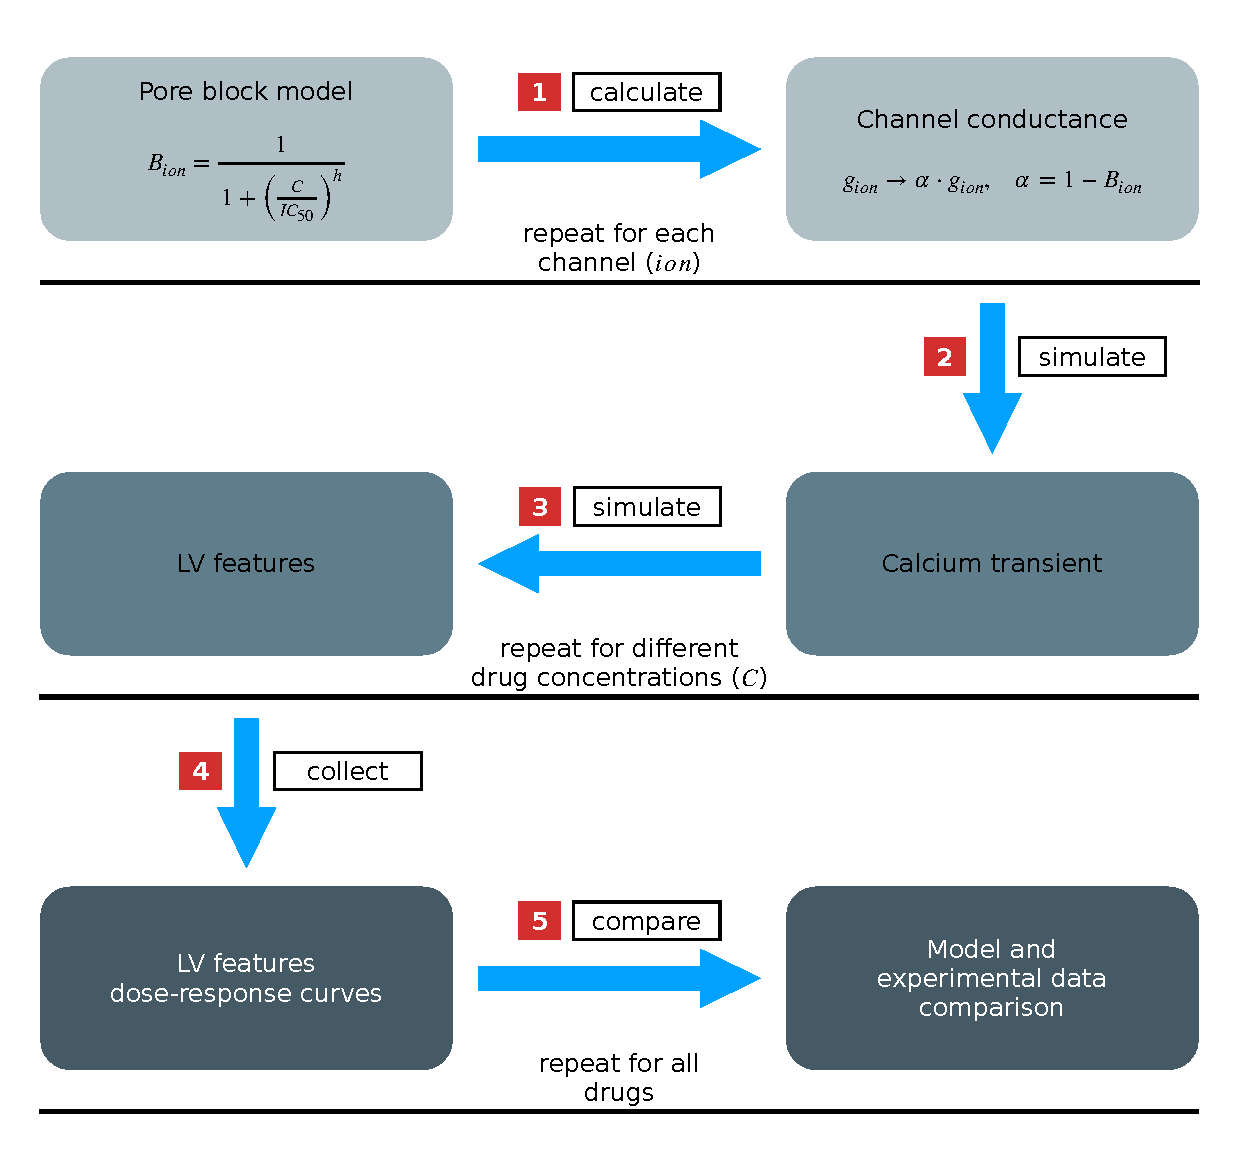
\includegraphics[width=\textwidth]{figures/chapter06/model_validation_schematic.pdf}
    \caption{Model validation workflow. (1) The pore block model is used to calculate the fraction of blocked ion channel at a given drug concentration for each ion channel. The same channels conductances are scaled to reflect this drug effect and (2) the rat myocyte electrophysiological model is run to generate perturbed calcium transients for different drug concentrations. (3) The calcium transients are used as an input for the $3$D biventricular rat heart contraction model and as many LV features' perturbed values are obtained as the number of input curves, which corresponds to the number of tested drug concentrations. (4) Each LV feature values are plotted against the tested drug concentrations to obtain dose-response curves. (5) The qualitative trend of the LV features after \textit{in silico} drug ``administration'' is compared with literature experimentally measured same drug effects on the same LV features for all the drugs under study.}
    \label{fig:validationschematic}
\end{figure}


%
%
%
\section{Results}\label{sec:ch6results}
A comparison of qualitative model predictions against experimental observations is shown in Fig.~\ref{fig:validationtable}. The model correctly predicted $16$ out of $19$ ($\SI{84}{\percent}$) experimental observations, with $5$ observations missing data, matching $6$ out of $8$ compounds. Model predictions were never opposite to observations, with either the model or observations reporting no-change when the model failed.

\begin{figure}[!ht]
    \myfloatalign
    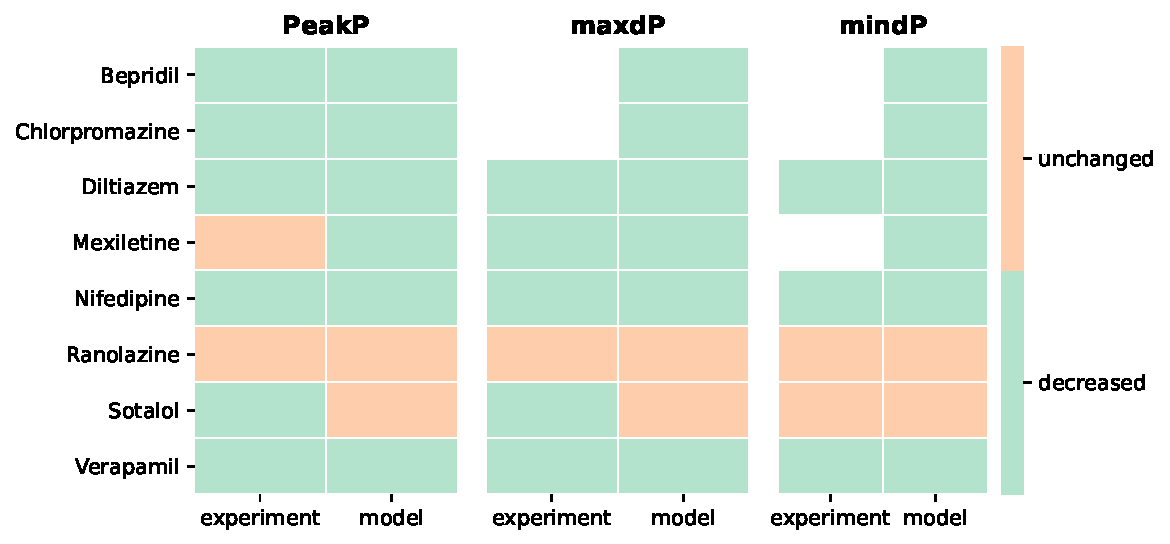
\includegraphics[width=1\textwidth]{figures/chapter06/model_vs_experiments.pdf}
    \caption{Model validation against known CiPA compounds effects on whole-organ function. Eight CiPA compounds effects (``experiment" columns) on PeakP, maxdP and mindP are compared with model same drugs' predicted effects on the same features (``model" columns). Drugs' effects are colour-coded as orange (feature unchanged) and green (feature decreased). None of the drugs caused an increase in the considered LV features. White/empty space means that the specific effect could not be retrieved from the examined literature studies. Model predicted effects are in agreement with the experimentally observed effects for $6$ out of $8$ compounds.}
    \label{fig:validationtable}
\end{figure}


%
%
%
\section{Discussion}\label{sec:ch6discussion}